\chapter{The PC2L Library}
The main contribution of this thesis is an easy-to-use library for distributed C++ that supports standard library algorithms. The library includes two data structures, \texttt{pc2l::Vector} and \texttt{pc2l::Map} which work the same way as their standard library equivalents. In order to relay information between machines on an interconnected computing cluster, MPI. A single write-back cache on the \texttt{CacheManager} node (MPI rank 0) is utilized, and memory is moved to the connected \texttt{CacheWorker} nodes as soon as the RAM space on the head node is exceeded. The code for the library is publicly available on github at \url{https://github.com/rudiejd/pc2l}, and it is intended to be used as a static shared library. Additionally, we have provided several applications which illustrate how PC2L might be used. Other than including some wind-up code which ensures that MPI is correctly initialized and terminated, data structures within the library can be used in exactly the same fashion as those in the libstdc++ STL.

\paragraph{Code sample}
This code solves the first project euler problem, which asks for the sum of all numbers below $n$ that are multiples of 3 or 5. \cite{euler_1}. Compare to the STAPL code mentioned in Chapter 2.
\scriptsize
\begin{lstlisting}[language=C++, caption=PC2L code sample for Project Euler number 1. Headers removed for brevity, captionpos=b]

using ull = unsigned long long;

int main(int argc, char *argv[]) {
    // Boilerplate code to get MPI up and running
    auto& pc2l = pc2l::System::get();
    pc2l.initialize(argc, argv);
    pc2l.start();
    ull num = strtoull(argv[1], NULL, 0);

    // initialize a vector of type unsigned long long filled with the number specified by 2nd command line argument
    // this vector uses blocks of size 8 * sizeof(ull) = 8 * 8 = 64 bytes (on most systems)
    // Note how this value can be provided by users
    pc2l::Vector<ull, 8 * sizeof(ull)> vec(num);

    // fill vector with values from 1 to n
    std::iota(vec.begin(), vec.end(), 1);

    // every number that does not have a 3 or 5 as a factor is set to 0
    std::replace_if(vec.begin(), vec.end(), [](auto i) {
        return !((i % 3) || (i % 5));
    }, 0);

    // sum all elements in the vector
    auto total = std::accumulate(vec.begin(), vec.end(), 0ULL);

    std::cout << "The total is " << total << std::endl;

    // Boilerplate to shut down MPI
    pc2l.stop();
    pc2l.finalize();
}
\end{lstlisting}
\normalsize
\section{Architecture}
\begin{figure}[h]
\centering
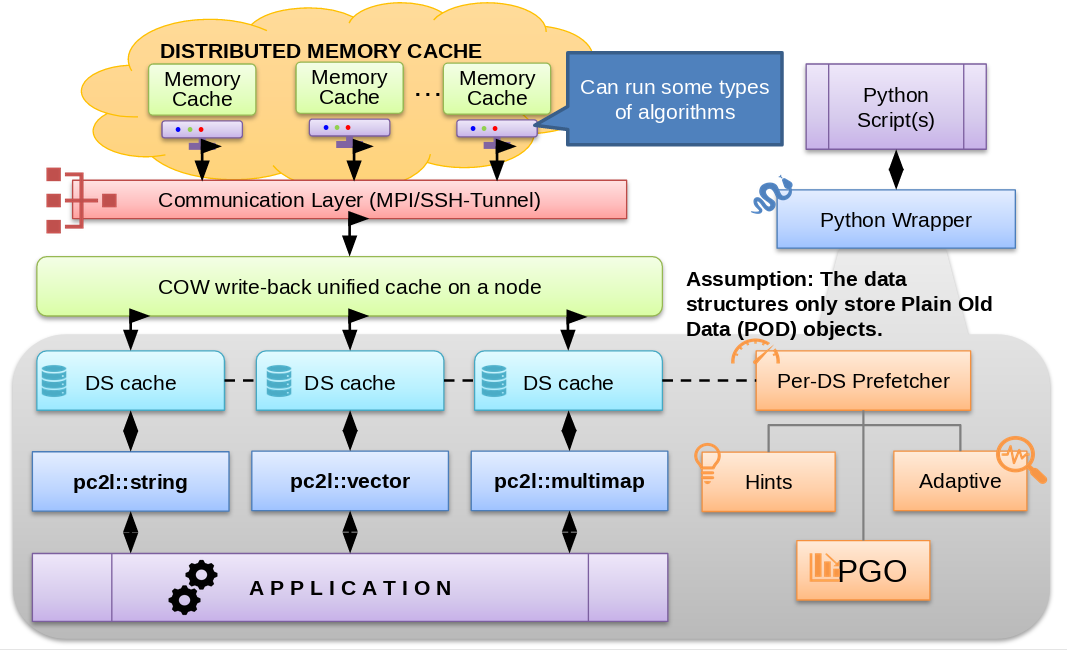
\includegraphics[width=0.65\textwidth]{Figures/pc2l_architecture.png}
\caption{Visualization of the difference from \cite{dist_java}. These red lines represent internal connections within a cluster. This is obviously a simplifcation, as all of these lines would likely be connected to a switch or some other communication mechanism.}
\label{fig:pc2l_architecture}
\end{figure}
As previously discussed, PC2L's architecture is based on a single "writer" node that serves as the cache along with networked child nodes that essentially operate in a write-back scheme. Figure \ref{fig:pc2l_architecture} displays the initial vision for how PC2L might have worked. As of the completion of this thesis,  only a COW write-back unified cache and a distributed memory cache accessed through a communication tunnel have been achieved. The data structures depicted in this initial vision have also been implemented, and some degree of rudimentary prefetching has been implemented. However, there is not currently a python wrapper for this project. We arrived at several important implementation decisions in the course of implementing this architecture including storing member data for each data structure in blocks of heterogeneous size, utilizing template metaprogramming not just for generic typing, but also to allow users to choose functionality for each data structure, custom cache eviction routines, and prefetching routines. Each one of these topics deserves more thorough exposition. 

\subsubsection{Block Division}
Every time an item within a PC2L data structure is retrieved or stored, there is a chance that it may need to be retrieved or sent to a remote node based on the current state of the head node. 
